\scanpage{182}
Si donc on veut trouver des op. coh. intéressantes via les opérations de $\Omega$
\unsure{de} $\Omega(k)$ sur la coh., il faut \unsure{ess.t|en.t}
se placer \uline{en car. $2$} (\unsure{en catimini|au contraire})
-- on peut espérer trouver alors une
description des \deleted{\unsure{op.}}\inserted{\unsure{carrés}}
de Steenrod mod $2$ (regarder ce qu'il en est \unsure{en|au}).

Mais on peut essayer d'être plus astucieux, en appliquant p.ex. le foncteur
\[
 \tau_\omega:(\operatorname{Mod\,grad}S_k\Rightarrow)M\longrightarrow M_\omega
\]
donc $X_*\longmapsto\operatorname{Hom}(X_*,\mathcal A_{k*}^{\unsure{\wedge}})$ devient un
foncteur sur (Semisimpl.) à valeurs
dans les objets \inserted{algèbres} gradués diff. de $\mathcal M_\omega$
(qui est une cat. de \unsure{tenseurs} ``\unsure{de car. $k$}'',
avec $\otimes$ comm.), et on peut se
proposer, \unsure{laissant} tomber la structure
graduée au profit de la structure
d'anneau diff. sous-jacent, de
déterminer le groupe des autom.
de ce foncteur (d'abord pour $k$ fixe,
puis sa variation avec $k$). Peut-être
trouverons nous des op. coh. intéressantes
notamment puiss. de Steenrod --
\margin{\uline{Non}}
\figure{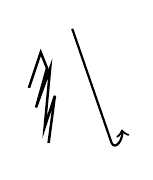
\begin{tikzpicture}
\draw[->,line width=.8pt] (0,1.6)--(.5,.15)..controls(.55,.05)and(.65,.2)..(.63,.32);
\draw[line width=.9pt] (-.55,.85)--(-.4,1.3)--(-.32,1.1)--(-.46,.6)--(-.28,1.1)--(-.35,.35)--(-.22,.75)--(-.3,.15);
\end{tikzpicture}}
\margin{181}
